\chapter{Eavesdropping attacks} \label{chap:eavesdropping_attacks}

\iffalse
    The whole attack could not be
    carried out, 
    
    Insist on the implementation and
    detailed explanation, this is the product. The whole attack could
    not be carried out. I think no publication shows how to do it and
    the only one was Munaut at 27C3. Really not trivial. try to explain
    the method and to give it a nice name. How i tried to solve the pb
    and implement the code
    \fi

    This chapter will focus on two eavesdropping attacks using
    \proj{OsmocomBB}: one on \gls{gsm}, the other on \gls{gprs}. The
    first section of the chapter explains the role of \proj{OsmocomBB}
    in the attack. It describes the way it was used to take a different
    approach to the problem by creating a passive listener exploiting
    dedicated hardware. The next sections are dedicated to the four
    steps of the attack.

    The first one consists of finding the location of the target, and
    the second one consists of finding its \gls{tmsi}. The \gls{tmsi}
    and location of the subscriber are linked, since the purpose of the
    \gls{tmsi} is to provide confidentiality to the subscriber by
    preventing attackers to track its location. Therefore, these two
    steps are also linked. The third step consists in finding the
    session key of the target. Encryption is applied by the network to
    provide data confidentiality, and to prevent eavesdropping. It is
    thus necessary to find this key to be able to eavesdrop on the
    communication. Finally, the last step is to capture this
    communication on the Um interface and to decode
    it~\cite{3gpp_ts_2006}.

    Various applications and commands of the \proj{OsmocomBB} project
    are detailed in this chapter. \Sref{app:tuto} of the appendices is
    available to describe their installation and usage. Some
    modifications were also done to these applications for the purpose
    of this thesis and some of them are described in context in this
    chapter. Explanations on how to apply these modifications are also
    available in the appendices.

  \section{\proj{OsmocomBB} as a passive listener}
  \label{sec:passive_listener}

    Before the availability of the \proj{OsmocomBB} project, the usual
    method to capture \gls{gsm} signals was to use an \gls{usrp} device
    combined with tools from the \proj{Airprobe} project. These tools,
    introduced in~\Sref{sec:airprobe}, were not optimal for several
    reasons. Firstly, this system could not effectively follow frequency
    hopping. Secondly, the received signal was a bit unreliable.
    Finally, capturing uplink traffic was complicated. The
    \proj{OsmocomBB} project is based on an actual mobile phone, which
    means that it uses hardware dedicated to \gls{gsm}. A mobile phone
    is designed to switch between frequencies very quickly, and to
    demodulate and decode uplink and downlink \gls{gsm} signals.
    Therefore, \proj{OsmocomBB} does not suffer from the same problems,
    and was a good candidate as a basis for an eavesdropping attack.

    Eavesdropping requires the attacker to break the encryption applied
    on the communication. A tool exists to find A5/1 session keys,
    \proj{Kraken}, but it expects some keystream generated using this
    key. Finding keystream requires to XOR a bitstream of plaintext and
    ciphertext. However, \proj{OsmocomBB} relies on the phone modem to
    produce layer 2 packets, as explained in~\Sref{sec:modem}. Since the
    encryption process is applied at a very low level, this does not
    give access to the encrypted keystream.

    For that purpose, \name{Sylvain Munaut} demonstrated at DeepSec 2010
    how it was possible to create a passive listener from one of the
    phones supported by \proj{OsmocomBB}, and to extract the bits off
    the air just after the demodulation and without further
    processing~\cite{munaut_cheap_2010}. This makes it possible to
    capture keystream to find the associated session key. It is also
    possible to use code from \proj{Airprobe} programs to convert these
    bits to upper layer packets. As a bonus, this listener supports
    uplink capture, can follow frequency hopping, has a very good
    demodulation, and is very inexpensive. 

    \begin{figure}[h]
      \centering
      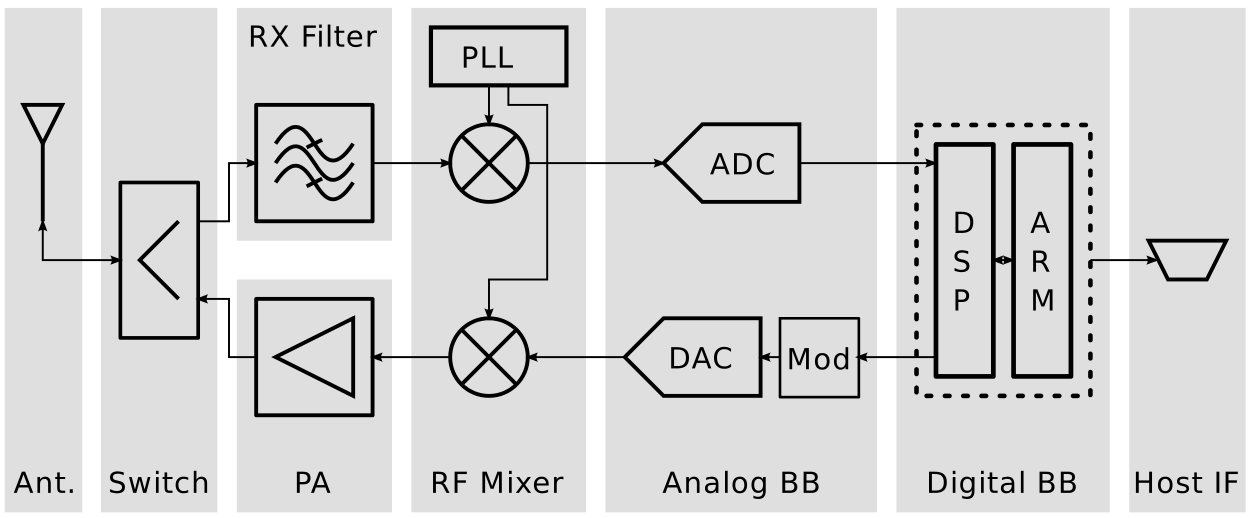
\includegraphics[width=\textwidth]{typical_calypso_platform}
      \caption{Block diagram of a typical Calypso
              platform~\cite{munaut_further_2012}}
      \label{fig:typical_calypso_platform}
    \end{figure}

    A simplified diagram of the receive and transmit path of a typical
    Calypso platform is shown on \fref{fig:typical_calypso_platform}.
    More information on that topic is available in~\Sref{sec:modem}.
    What interests us here is the upper part of the figure: the
    receive path. It is composed of several components and each of
    them could be an obstacle to the implementation of the listener.

    \begin{itemize}[topsep=-1em,parsep=0em,itemsep=0.5em]

      \item The antenna is completely common. In case of uplink capture,
        it could be replaced by another antenna, but it is not really
        necessary.

      \item The antenna switch splits the signal between the receive
        path and the transmit path, and does not cause any problem.

      \item The reception filter reduces the noise by attenuating every
        signal which is not at the received downlink frequency by around
        \SI{35}{\deci\bel}. This means that it strongly attenuates the
        received uplink signal which is already weak. It can be replaced
        to increase the uplink reception range from less than
        \SI{20}{\meter} to around \SI{150}{\meter}, but the operation is
        delicate due to the components size.

      \item The \gls{rf} mixer tunes the phone to any frequency in the
        four downlink bands. The uplink bands are out of the
        specifications, but after removing the dedicated verification
        functions, the \gls{pll} can be configured to support them as
        well. Of course, the results are a bit poorer, but not
        significantly. The mixer also needs to be configured to deal with at
        least two consecutive bursts instead of one, to receive the
        uplink as well. This is possible since multislot is a feature of
        \gls{gprs} which is supported by the Calypso
        platform.

      \item The analog baseband is simply an \gls{adc} in this case, and
        the demodulation is done in the \gls{dsp}. It receives I/Q
        symbols and converts them to digital samples coded as soft
        bits.

      \item The first part of the digital baseband is the \gls{dsp}.
        When used in normal operation, it processes the digital signal
        to reconstruct a layer 2 packet. The traffic bursts are
        decompressed inside the \gls{dsp} and sent directly to the audio
        codec. The \gls{dsp} firmware is stored in a mask \gls{rom}, but
        part of the \gls{ram} can be used to patch it. This is done by
        overwriting entries in a function table to provide new functions
        stored in \gls{ram}. The new functions modify the \gls{dsp}
        behavior to send the demodulated bits to the second part of the
        digital baseband without further processing.

      \item The second part of the digital baseband is an ARM processor
        which hosts the \proj{OsmocomBB} firmware. This makes it easier
        to apply the four necessary modifications. The first is to use
        the \gls{dsp} bootloader to patch the \gls{rom} and provide the
        functions for the sniffing task in \gls{ram}. The second is to
        add this task to the \gls{dsp} driver. The third is to use it in
        the \gls{dsp} to get the raw demodulated bits. The last is to
        replace data transmission by the reception of the uplink
        frequency using the same task.

      \item The last component is the serial interface used to
        communicate with the host computer. After the modifications in
        the receiving path, it has to transmit 4 bursts of 116 soft bits
        every \SI{4.615}{\milli\second}, which requires non standard
        baud rates.\fxnote{Why four and not two? Because it might be
        useful in the future?}

    \end{itemize}

    After all these modifications, the listener is able to receive the
    demodulated bursts in up to four time slots per frame, for the
    downlink or the uplink. These are saved in a file that can be
    decoded using parts of the programs available in \proj{Airprobe}. To
    summarize, the impact of this \proj{OsmocomBB} based passive
    listener comes from its good uplink support, its hardware dedicated
    to frequency hopping and \gls{gsm} signal processing, and its wide
    availability. The modifications applied to \proj{OsmocomBB} to
    create a passive listener are available in the
    \code{sylvain/burst\_ind} branch of the project git repository. The
    filter replacement, as well as the choice of a suitable USB to RS232
    converter, is described on the project website.

    An example of the output of a modified version of the
    \prog{ccch\_scan} application is shown on \fref{fig:log_bi}. This
    application is intended as a small demonstration of what is possible
    using this passive listener. The \gls{ms} will follow any Immediate
    Assignment message to the dedicated channel, and will save all the
    relevant bursts to a file. On the figure, four bursts received in
    four consecutive frames are highlighted twice: once for the
    downlink, and once for the uplink. The layer 2 message is contained
    into these four bursts due to the interleaving process. Once the
    four bursts are received, they are deinterleaved and decoded to a
    layer 2 message, which is sent to \proj{Wireshark} via
    \prog{gsmtap}.

    \begin{figure}[h]
      \centering
      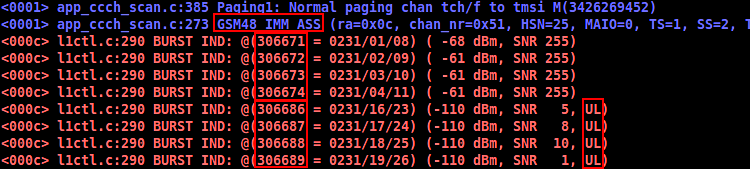
\includegraphics[width=\textwidth]{log_bi}
      \caption{Output of the \prog{ccch\_scan} application in the
        \code{burst\_ind} branch.\fxnote{cfr gsm time!}}
      \label{fig:log_bi}
    \end{figure}

    \iffalse On Mon, Aug 29, 2011 at 01:55:59AM +0200, Lukas Kuzmiak
    wrote: > If I'm not mistaken pl2303 based cables have/had problems
    handling baudrates > above 115200, there was a recent update into
    the kernel tree, but I've never > tested it.

the problem is not "[standard] baud rates above 115200" but it is
"non-standard baud-rates at all".  Normal USARTs have baud-rate
generators that can only generate baud-rates "input_clock / divider"
where divider is either an integer, or even more: limited to a power of
2

The calypso cannot do any standard baud-rates above 115200.  That's why
you need a USART with more flexible baud rate generator.  The most
commonly known one to do this is the FTDI series of USB-serial
converters. 
    \fi

  \section{Recovering the location}

    After describing how to create a passive listener, the details of
    the attack itself will be investigated. The attacker needs to be in
    the same cell as the targeted phone since everything happens on the
    Um interface. If the location of the target is not known, it is
    possible to exploit the \gls{ss7} to find relevant information. The
    \gls{ss7} contains various protocols that are used in the telephony
    world. One of them, the \gls{map}, was designed to provide signaling
    services between various elements of the mobile networks and is
    introduced in~\Sref{sec:ss7}. Two services described there can be
    exploited to get location information for a given subscriber if an
    access to the network is available.

    \subsection{Accessing the SS7 MAP protocol}

      According to \name{James Moran}, the security director for the
      \gls{gsma}: \textquote{SS7 is inherently insecure, and it was
      never designed to be secure}~\cite{timberg_for_2014}. This makes
      it difficult for the operators to prevent abuses. Nevertheless,
      good filtering policies could reduce the attack surface but, at
      the end of 2014, \name{Karsten Nohl} said that many operators do
      not implement them. Moreover, some \gls{ss7} services are needed
      for normal network operation, and thus are almost impossible to
      filter. This allows anyone with a roaming agreement and an access
      to the \gls{ss7} to request this
      information~\cite{nohl_mobile_2014}.

      According to \name{Tobias Engel}, \textquote{getting access to the
      SS7 is easier than ever}, and since legitimate commercial services
      need it, it \textquote{can be bought from telecom operators or
      roaming hubs for a few hundred euros a month}. He also said that
      \textquote{some network operators leave their equipment unsecured
      on the Internet}. Another access vector could be femtocells.
      Indeed, since they are part of the core networks but placed in
      subscribers homes, it could be possible to hack them to get an
      access~\cite{engel_ss7:_2014}.

    \subsection{HLR query}
    \label{sssection:hlr_query}

      An \gls{hlr} query is a name commonly used for a
      MAP-SEND-ROUTING-INFO-FOR-SM service request, which is described
      in more details in~\Sref{sec:sriforsm}. A way of exploiting this
      service was presented by \name{Tobias Engel} at the
      25C3~\cite{engel_locating_2008}.

      It is easy to see on \fref{fig:map_srifs_hl} that during a
      legitimate \gls{sms} delivery procedure, the \gls{gmsc} requests
      information from the \gls{hlr}, and then sends the \gls{sms}
      message on its own. This can be exploited because the fourth step on
      the diagram is actually optional. Having access to the \gls{ss7},
      it is therefore possible to request information from the \gls{hlr}
      and never send any \gls{sms} message. The information returned is,
      based on a subscriber phone number, the \gls{imsi} of the
      subscriber as well as the number of the \gls{msc} serving it.

      \begin{figure}[h]
        \centering
        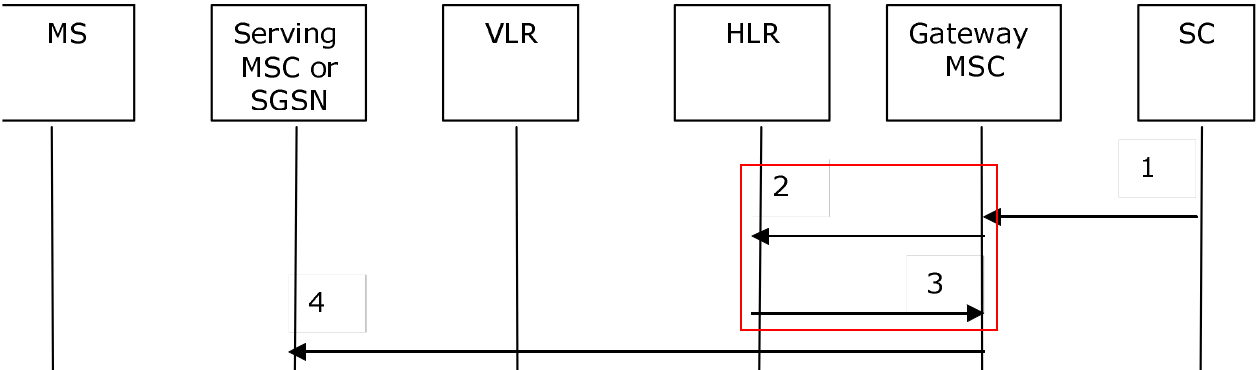
\includegraphics[width=\textwidth]{map_srifs_hl}
        \caption{Exploiting the MT-SMS
      procedure~\cite[p.~792]{3gpp_ts_2015-2}.}
        \label{fig:map_srifs_hl}
      \end{figure}

      %http://www.nkom.no/npt/numsys/E.164.pdf
      The number of the \gls{msc} gives information on the current
      location of the mobile phone, since it starts with a country code.
      It also gives information on the operator to which the phone is
      currently connected to thanks to its identification code. The
      result of an \gls{hlr} query displaying the number of the
      \gls{msc} is shown on \fref{fig:location}. On this example, the
      country code, 47, belongs to Norway, and the identification code,
      92, belongs to \comp{Netcom}~\cite{nkom}.

      \begin{figure}[h]
        \centering
        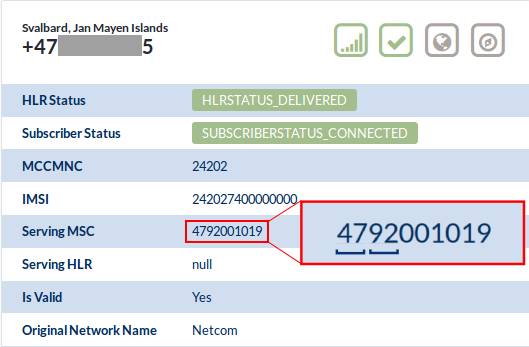
\includegraphics[width=\textwidth]{location}
        \caption{MSC number returned from an HLR query.}
        \label{fig:location}
      \end{figure}
      
      These \gls{hlr} queries allow to build databases providing a
      mapping between an \gls{msc} number and a location by querying
      phones in known locations. An example presented by
      \name{Tobias Engel} for Germany is shown on
      \fref{fig:location_te}. The area that an \gls{msc} covers might be
      a part of a city, a whole city or even bigger. Indeed, an
      \gls{msc} usually handles a certain amount of traffic and
      therefore the area it covers depends on the population density.
      Thus, determining the \gls{msc} where the phone is located is only
      a first step to uncover the location of the targeted phone.

      \begin{figure}[h]
        \centering
        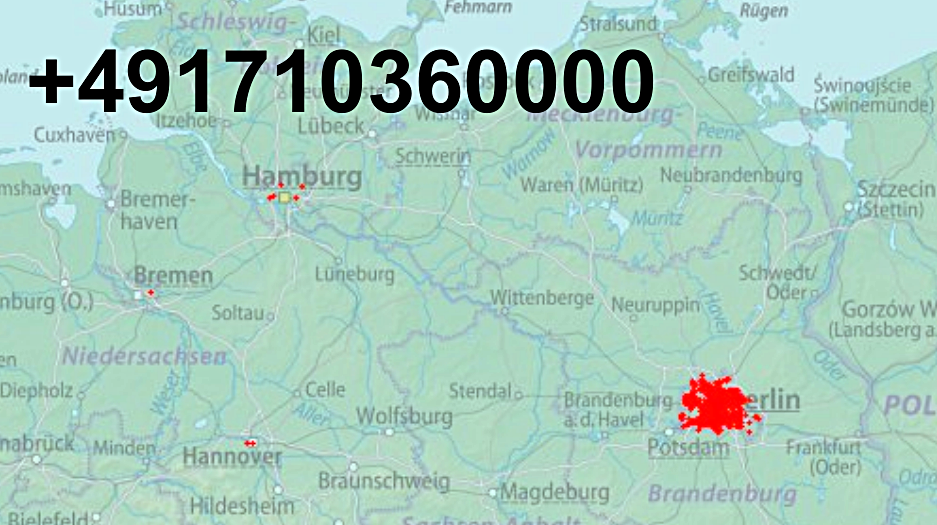
\includegraphics[width=\textwidth]{location_te}
        \caption{Mapping between MSC numbers and
        location~\cite{engel_locating_2008}}
        \label{fig:location_te}
      \end{figure}

      To find the cell of interest, two methods can be used. Either
      wardriving, which is explained in \Sref{sec:recovering_tmsi},
      or a \gls{psi} service request. While it is easy to find companies
      providing cheap and easy to use \gls{hlr} queries online,
      \gls{psi} requests are more difficult to access.

    \subsection{MAP PSI service}

      PSI service is a short name for the MAP-PROVIDE-SUBSCRIBER-Info
      service described in~\Sref{sec:psi}. At the 31C3, \name{Karsten
      Nohl} showed how it was possible to exploit it to recover a more
      precise location than with an \gls{hlr} query
      alone~\cite{nohl_mobile_2014}. Indeed, an \gls{hlr} query gives
      the \gls{imsi} of the subscriber based on its phone number, while
      a PSI service request gives the \gls{cgi} related to this
      \gls{imsi}. The \gls{cgi} is composed of the \gls{mcc}, the
      \gls{mnc}, the \gls{lac}, and the Cell ID, as explained in
      \Sref{sec:cgi}. This allows one to easily find the location of the
      target by querying one of the Cell ID database available online.

    \section{Recovering the TMSI}
    \label{sec:recovering_tmsi}
      
      The previous step gave out the location of the target and the cell
      it is camping on. It is now necessary to find out the identity of
      the target on this cell to be able to follow its calls on the
      dedicated channel. The \gls{tmsi} can not be queried over the
      \gls{ss7} \gls{map} protocol, so another method is used to recover
      it.
      
      It works by contacting the targeted phone according to a given
      pattern and by listening to the beacon channel looking for a
      \gls{tmsi} getting paged according to the same pattern. This makes
      the assumption that the \gls{tmsi} will stay the same between the
      beginning and the end of the process. Listening to the beacon
      channel can be done with a mobile phone using the
      \code{ccch\_scan} application available in \proj{OsmocomBB}. An
      example of its output is shown on \fref{fig:log_tmsi}.

      \begin{figure}[h]
        \centering
        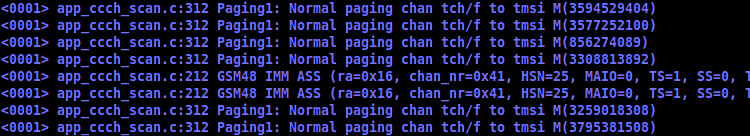
\includegraphics[width=\textwidth]{log_tmsi}
      \caption{Output of the \prog{ccch\_scan} application.}
        \label{fig:log_tmsi}
      \end{figure}

      This method can also be used to refine the location granularity
      after a simple \gls{hlr} query. Every paging request is sent on
      the whole location area, so by looking for the pagings in each of
      the location area served by the serving \gls{msc}, it is possible
      to determine if the targeted phone is there or not. The same
      method can be applied to find the \gls{cgi}. The attacker can go
      from one cell to another and look for the paging responses sent by
      the targeted \gls{tmsi}, to make sure to be in the right cell.
      This is called wardriving.

      To make sure that the user of the targeted phone does not notice
      this step, it is possible to send so called silent \gls{sms}
      messages, which are not displayed on the targeted
      phone~\cite[p.~53]{3gpp_ts_2001}. If they are blocked by the
      operator, it is also possible to send broken \gls{sms} messages
      that the mobile discards but this is dependent of the baseband
      implementation~\cite{golde_sms-o-death:_2011}. A last method
      consists of initiating a phone call, and hanging up after the
      paging is done, but before the user is
      alerted~\cite{kune_location_2012}.

      An implementation of the silent \gls{sms} feature is proposed with
      this thesis. Each \gls{sms} message contains a
      TP-Protocol-Identifier field, and setting its value to \code{0x40}
      tells the receiving \gls{ms} to discard its contents. This means
      that the targeted \gls{ms} is paged, but that nothing shows up on
      the targeted user's screen. This is called a type 0 \gls{sms}.
      Another field that can be modified is the TP-Data-Coding-Scheme
      field, which indicates whether or not an \gls{sms} message is
      compressed. It consists of two bytes, and if the first byte is set
      to \code{0xC0}, the \gls{ms} may discard the contents of the
      message~\cite[p.~6]{etsi_gsm_1999}. The patch can be found in the
      appendices \Sref{app:patches} and provides the \prog{silent}
      command in the \prog{mobile} application of \proj{OsmocomBB}, as
      displayed in \fref{fig:mobile_silent}. An implementation of the
      correlation feature could not be developed since Norwegian
      networks reallocate the \gls{tmsi} too often, as discussed
      in~\Sref{sec:tmsi_realloc}.

      \begin{figure}[h]
        \centering
        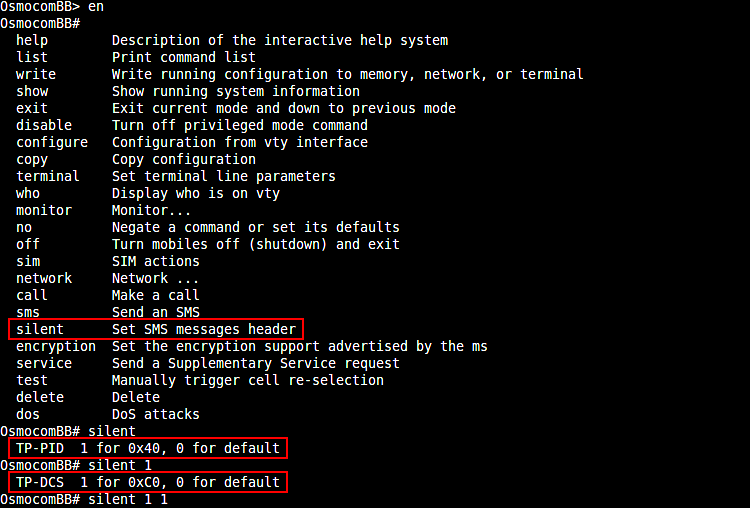
\includegraphics[width=\textwidth]{mobile_silent}
        \caption{Set TP-PID and TP-DCS fields using the patched
        \prog{mobile} application}
        \label{fig:mobile_silent}
      \end{figure}
      
    \section{Finding the session key}
    \label{sec:finding_kc}

      Once the location and identity of the target are found, it is
      necessary to uncover the session key before being able to capture
      a call. This is needed to decrypt the traffic of course, but also
      to find out the frequencies on which the traffic is sent. Indeed,
      the traffic channel is assigned by an Assignment Command sent on
      the dedicated channel after enabling the encryption, as explained
      in \Sref{sec:rr_proc}. The session key needs to be found before
      the Assignment Command to be able to capture the beginning of the
      call as well. To do so, it is necessary to capture data on the Um
      interface, including the communication and the keystream, and to
      decode it.

      \subsection{Capturing keystream and using \proj{Kraken}}

      The first way of solving this problem makes two assumptions.
      Firstly, the encryption algorithm has to be A5/1 or A5/2, because
      they are broken. Secondly, there should not be any key
      renegotiation between the discovery of the key and the targeted
      call. Some networks assign a session key to be used several times,
      but other renegotiate a new key more often. If the key is
      renegotiated after every \gls{sms} message, this method is
      useless.

      If these assumptions are met, the first step is to page the target
      using one of the method discussed in the previous section, silent
      \gls{sms} messages for example. Since they are sent encrypted on
      the dedicated channel, it is possible to follow them and capture
      some keystream using the passive listener described
      in~\Sref{sec:passive_listener}. Indeed, there is a lot of known
      plaintext in \gls{gsm}. For example, the System Information 5 or 6
      can be found encrypted and unencrypted, as shown on
      \fref{fig:si5_keystream_ws}~\cite{nohl_gsm:_2009}.

        \begin{figure}[h]
          \centering
          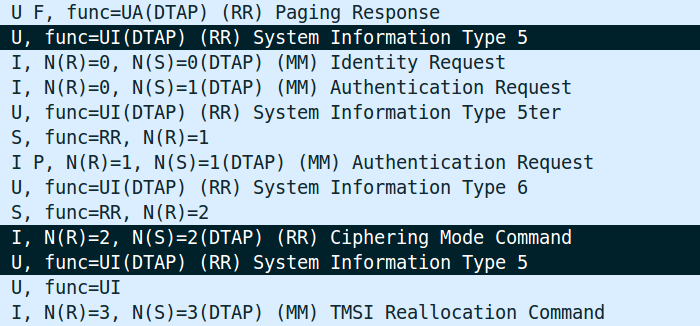
\includegraphics[width=\textwidth]{si5_keystream_ws}
          \caption{SI5 sent before and after the Ciphering Mode Command}
          \label{fig:si5_keystream_ws}
        \end{figure}

      The keystream associated with the session key can be recovered
      with a XOR operation on the plaintext and the ciphertext. That
      keystream can then be used to find the session key using
      \proj{Kraken} along with the Berlin table set described in
      \Sref{sec:berlin}, and this session key can serve to follow the
      next phone call, as long as the key did not change.

      Finding keystream can be done with a program proposed with this
      thesis. The patch is available in \Sref{app:keystream} of the
      appendices, and modifies a version of the \prog{ccch\_scan}
      application found in the \code{sylvain/burst\_ind} branch. This
      modified application will follow a given \gls{tmsi} on the
      dedicated channel, and store the plaintext of a System Information
      5 message sent before the Ciphering Mode Command. When the
      encryption is started, it will then try to guess which encrypted
      message is a System Information 5 message based on a sequence
      provided by the user. Finally, it outputs potential keystream by
      applying a XOR operation on the stored plaintext and the
      ciphertext. Its usage is described in the appendices, and an
      example of its output is shown in \fref{fig:keystream}.

        \begin{figure}[h]
          \centering
          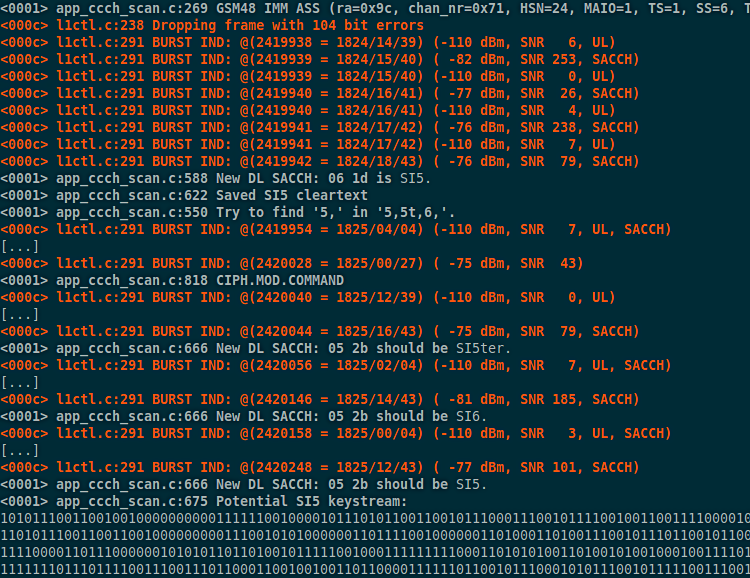
\includegraphics[width=\textwidth]{keystream}
          \caption{Output of the modified \prog{ccch\_scan} application
          in the \code{burst\_ind} branch displaying potential
        keystream}
          \label{fig:keystream}
        \end{figure}

      \subsection{MAP Send Identification service}

        A second way of finding the session key exists, which gets rid of
        the previously mentioned assumptions, as long as an access to
        the \gls{ss7} \gls{map} protocol is possible. Firstly, this
        method can provide session keys regardless of the encryption
        algorithm used, even A5/3. Secondly, there is no risk of
        triggering a session key renegotiation simply by using it. This
        technique exploits the MAP\_SEND\_IDENTIFICATION service described
        in~\Sref{sec:si}.

        The request associated with this service can be used to recover
        the session key associated with a \gls{tmsi}, as well as up to
        five authentication sets. The authentication sets, or
        authentication triplets, contain the random challenge, the
        signed response, and the session key for the following
        sessions~\cite[p.~100]{3gpp_ts_2015-1}. Exploitation of this
        service request make the encryption on the Um interface
        irrelevant.

    \section{GSM eavesdropping}

      After describing various ways of recovering the location,
      \gls{tmsi}, and session key of the target, this section will focus
      on the actual call capture and explain how to use the passive
      listener described in \Sref{sec:passive_listener} to create a
      sniffer.

      A sniffer needs to be able to record mobile-terminating services
      as well as mobile-originating ones. When the targeted phone
      initiates a call, there is no paging on the beacon channel since
      the phone sends a request directly. This makes it impossible for
      the sniffer to follow the target on the dedicated channel by
      listening to the paging messages only. This problem is solved by
      following every Immediate Assignment message seen on the beacon
      channel to the dedicated channel. If this Immediate Assignment
      was not addressed to the targeted phone, messages after the
      Ciphering Mode Command could not be decrypted with the session key
      found earlier. If these messages can be decrypted, then the
      Assignment Command is followed to the traffic channel and the call
      recorded.

      On a busy cell, it is common for Immediate Assignment messages to
      be sent very close to each other. The interval can be smaller
      than the time needed for the listener to realize that the
      Immediate Assignment message was not relevant and to synchronize
      on the beacon channel again. Therefore, several listeners are
      needed to build a sniffer capable of processing all the
      assignments messages. To do so, one listener can stick to the
      beacon channel and coordinate the others by assigning them to a
      dedicated channel in turn. The more listeners are available, the
      more Immediate Assignment messages can be followed in parallel.

      When the raw demodulated traffic bursts are saved in a file, a
      program based on \proj{Airprobe} can decode them to audio. This
      means that, under certain conditions, it is possible to eavesdrop
      on the downlink and the uplink of a hopping \gls{gsm} phone calls
      for less than \SI{1500}{kr} or \SI{200}{\euro}.

    \section{GPRS eavesdropping}

      At the Chaos Computer Camp in 2011, \name{Luca Melette} and
      \name{Karsten Nohl} showed how it was possible to use the same
      passive listener as a basis to listen to \gls{gprs} signals as
      well~\cite{melette_gprs_2011}. It seems to be the only public
      attack of this kind, but it is more of a demonstration of what is
      possible and not as complete as what can be done for \gls{gsm}.
      Thus, several steps are missing. For example, the recovery of the
      temporary identity or the session key was not
      shown~\cite{srlabs_gprs_????}.

      Because it is complicated to find all the \gls{gprs} packets, this
      demonstration only works on a single \gls{arfcn} and captures all
      the time slots from the uplink or downlink frames on one channel.
      It uses two listeners to do so, since each of them is able to
      listen to four time slots per frame.

      To decode the captured demodulated raw bits, a new program was
      created: \prog{gprsdecode}. It multiplexes the data from the
      various time slots, then decodes it to the \gls{llc} layer and
      sends it to \proj{Wireshark}, where IP packets can be read. Since
      the \gls{gea} encryption used in \gls{gprs} is not broken yet,
      this only works for unencrypted traffic. Surprisingly, some
      networks did not encrypt traffic at the time of the
      presentation.\fxnote{what about psi requests to get the key?}

  \iffalse

  encryption ss7 : MAP_SEND_AUTHENTICATION_INFO service

  http://baseband-devel.722152.n3.nabble.com/GPRS-Vs-EDGE-Trying-to-decode-my-own-sessions-td3288960.html

  http://baseband-devel.722152.n3.nabble.com/uplink-sniffing-td3531044.html

  http://baseband-devel.722152.n3.nabble.com/GPRS-decode-tutorial-td3437051.html

  http://baseband-devel.722152.n3.nabble.com/Sniffing-GPRS-td3712433.html

  http://baseband-devel.722152.n3.nabble.com/Sniffing-GPRS-td3712433.html

  http://baseband-devel.722152.n3.nabble.com/Working-of-ccch-scan-and-capturing-the-SDCCH-td4025206.html#a4025213

  \fi
